% Supplementary Information (standalone), aligned with main.tex (sagej).
\documentclass[Afour,sageh,times]{sagej}

\usepackage{moreverb,url}
\usepackage{amsmath,amssymb}
\usepackage{graphicx}
\usepackage{xr-hyper}
\usepackage[colorlinks,bookmarksopen,bookmarksnumbered,citecolor=red,urlcolor=red]{hyperref}
% Prefix avoids clashing with sagej's FirstPage/LastPage labels in this document's own .aux.
\externaldocument[main-]{main}

\def\volumeyear{2026}

% Prefix labels with S to distinguish from the main text.
\renewcommand{\thesection}{S\arabic{section}}
\renewcommand{\theequation}{S\arabic{equation}}
\renewcommand{\thefigure}{S\arabic{figure}}
\renewcommand{\thetable}{S\arabic{table}}

\begin{document}

\runninghead{Correig-Fraga (Supplementary Information)}

\title{Supplementary Information for\\[0.5ex]
\itshape An attractor account of numerosity perception}

\author{Eudald Correig-Fraga\affilnum{1}}

\affiliation{%
\affilnum{1}Innovamat Education, Avinguda de la Generalitat, 217, Catalonia (Spain)}

\corrauth{Eudald Correig-Fraga, Innovamat Education, Avinguda de la Generalitat, 217, Catalonia (Spain).}

\email{eudald.correig@innovamat.com}

\maketitle

\noindent This document accompanies the article \emph{An attractor account of numerosity perception}. Supplementary Material~1 details the trial-level fitting; Supplementary Material~2 reports the full model comparison and the constrained cross-duration fits; Supplementary Material~3 the parameter recovery; Supplementary Material~4 the resolution-limit prediction and its robustness; and Supplementary Material~5 the exploratory developmental-dyscalculia reanalysis.

\section{Supplementary Material 1: Trial-level fitting}
\label{sm:methods}

\paragraph{Data.} We reconstruct one row per trial from the openly available data of~\citet{cheyette_unified_2020}, grouping by participant and trial and keeping the presented numerosity, the typed response, and the response time (converted to seconds). We use the five DURATION conditions (40, 80, 160, 320, 640~ms), true numerosities $n = 1$--$15$, giving ${\approx}10{,}600$ trials per duration and ${\approx}53{,}000$ in total. No trials are aggregated: the likelihood is evaluated over the individual integer reports.

\paragraph{Response likelihood.} For each model and duration the response probability of Eq.~(\ref{main-eq:marginal}) marginalises the readout over the sensory channel $y_0 \sim \mathcal{N}(n, \sigma(n))$. The integral is computed \emph{deterministically}, so the objective is free of Monte-Carlo noise. Gauss--Hermite quadrature is inappropriate here: for the attractor models the clean-up map $y_0 \mapsto x^*$ is near-discontinuous (evidence snaps to basins), and Gauss--Hermite carries a $1.7$--$4\%$ error even at $241$ nodes. We therefore use a uniform standard-normal grid with Gaussian weights for \emph{every} model, so the comparison is on identical footing; validated against high-sample Monte-Carlo, a grid of $801$ nodes matches to $\le 2\times10^{-3}$ (mean $1.5\times10^{-4}$). The optimiser uses a cheaper grid ($201$ nodes); the reported log-likelihoods are recomputed at the fitted parameters on a fine grid ($1601$ nodes).

\paragraph{Lapse channel.} Typed responses run up to $99$, and a few per cent of guesses fall outside the integer-well support ($3.9$--$6.1\%$ across durations). We never discard them: the final response probability is $p_{\mathrm{final}}(r \mid n) = (1-\ell)\,p(r \mid n) + \ell\,/\,R_{\max}$ with $R_{\max} = 99$, a uniform contamination that places positive mass everywhere. The lapse $\ell$ is fitted per duration under an identical convention across all models and is counted in AIC/BIC; it is stable across models (${\approx}0.06$--$0.08$).

\paragraph{Response-time and joint channels.} Response time is modelled as log-normal, $\log \mathrm{rt} \sim \mathcal{N}(\log(t_0 + m(n)), \sigma_{\mathrm{rt}})$, with the task-fixed base $t_0 = 1.30$~s. The metric $m(n)$ is the expected posterior entropy ($\kappa\,\mathbb{E}[H]$, available to every model), the expected convergence time ($\tau\,\mathbb{E}[T]$, attractor only), or their sum (the hybrid; Eq.~\ref{main-eq:rt}). Because the log-normal maximum-likelihood fit targets the mean of $\log \mathrm{rt}$, i.e.\ the geometric-mean RT, all reported $R^2$ values compare the prediction against the geometric mean rather than the median. The coupled joint $p(r, \mathrm{rt} \mid n)$ integrates response and RT over the same latent nodes; co-optimising all channels together (warm-started from the two-stage fit) leaves the model ranking unchanged and moves the landscape negligibly, so RT can be treated as a downstream cross-prediction.

\paragraph{Optimisation.} The deterministic objective is minimised by \texttt{scipy} differential evolution~\citep{storn_differential_1997} followed by a Nelder--Mead polish, with fixed seeds. The attractor models require a larger optimiser budget than the smooth static readouts (a low-budget fit understates them); re-fitting at a higher budget with a different seed changes the reported log-likelihoods by less than one part in $10^3$, confirming the fits are converged and the model ordering is not an optimisation artefact.

\section{Supplementary Material 2: Model comparison and constrained fits}
\label{sm:comparison}

Table~\ref{tab:ladder} gives the full trial-level response comparison. Every model is fitted under the identical convention (per-duration parameters plus a per-duration lapse, summed over the five durations). The super-linear-width Gaussian attractor is the best account; the ranking isolates the two ingredients that matter.

\begin{table}[t]
  \centering
  \caption{\textbf{Trial-level response model comparison.} Categorical information criteria over the ${\sim}53{,}000$ individual responses, summed over the five exposure durations, relative to the best model. $k$ is the total free-parameter count (per-duration mechanism parameters plus lapse). ``Attractor'' includes the clean-up dynamics; ``readout'' is the matched static control at the same $k$. The width-model rows carry one parameter more than the Weber/ANS and normative benchmarks (the free width exponent); at this sample size BIC charges ${\approx}9$ per parameter against AIC's $2$, yet the ranking and margins barely change, so the advantage is not a parameter-count artefact.}
  \label{tab:ladder}
  \setlength{\tabcolsep}{5pt}
  \begin{tabular}{lccc}
  \hline
  Model & $k$ & $\Delta$AIC & $\Delta$BIC \\
  \hline
  \textbf{Super-linear attractor (free $\beta$)} & \textbf{25} & \textbf{0} & \textbf{0} \\
  Super-linear attractor (power-law $n^{p}$) & 25 & 165 & 165 \\
  Super-linear readout (free $\beta$, static) & 25 & 1256 & 1256 \\
  Power-law readout (static) & 25 & 1491 & 1491 \\
  Weber/ANS ($\sigma_n \propto n$) & 20 & 4435 & 4398 \\
  Normative log-prior proxy & 20 & 7666 & 7629 \\
  \hline
  \end{tabular}
\end{table}

\paragraph{Clean-up at equal parameters.} Turning the clean-up dynamics on is a zero-parameter change (the dynamics are deterministic given the landscape), so the attractor and its static twin occupy the identical parameter space. Within the super-linear family this flips the fit by $\Delta\mathrm{AIC} = 1256$ in favour of clean-up, and within the power-law family by $1326$, showing that the dynamics do explanatory work rather than add flexibility. (Per duration, clean-up helps strongly at 40--160~ms and is roughly neutral at 320--640~ms, where the attractor has largely settled during the exposure itself.)

\paragraph{Width scaling.} The width exponent is a free parameter of the model rather than a fixed value. It is estimated firmly super-linear at every exposure except the noise-dominated 40~ms flash (Table~\ref{tab:params}), which gives the wells their sharp-to-broad profile: narrow and well-separated for small numbers, wide and overlapping for large ones. Granting the Weber/ANS code the same flexibility does not close the gap: freeing its width exponent (the power-law readout, also $k = 25$) leaves it $1491$ behind the winning attractor, and the freed exponent settles super-linear rather than at the Weber value $\sigma_n \propto n$, so at equal parameter count a magnitude code still loses and does not prefer the Weber scaling.

\begin{table}[t]
  \centering
  \caption{\textbf{Fitted parameters of the winning model across exposure durations.} $\sigma_c$ and $\beta$ set the well-width law $\sigma_n = (\sigma_c/f_n)^\beta$; $s_0$ and $\lambda_0$ the sensory-noise profile $\sigma(n)$; $\ell$ the lapse. The 40~ms flash is noise-dominated (large $s_0$, extreme $\beta$); from 80~ms the parameters vary smoothly.}
  \label{tab:params}
  \setlength{\tabcolsep}{4pt}
  \begin{tabular}{lccccc}
  \hline
  Duration & $\sigma_c$ & $s_0$ & $\lambda_0$ & $\beta$ & $\ell$ \\
  \hline
  40\,ms  & 0.085 & 0.023 & 2.91 & 3.42 & 0.080 \\
  80\,ms  & 0.054 & 0.0056 & 3.03 & 1.81 & 0.064 \\
  160\,ms & 0.047 & 0.0023 & 3.25 & 2.02 & 0.059 \\
  320\,ms & 0.045 & 0.00047 & 3.76 & 2.19 & 0.079 \\
  640\,ms & 0.041 & 0.00036 & 3.67 & 2.15 & 0.072 \\
  \hline
  \end{tabular}
\end{table}

\paragraph{Is the landscape stable across durations?} The main text fits each duration independently and reads the resulting parameter trajectories; the substantive finding is that the landscape sharpens with exposure ($n_{\mathrm{crit}}$ grows; Supplementary Material~4). As a backstop we also fitted constrained models that share the landscape parameters ($\sigma_c$, $\beta$) across durations, leaving only the sensory channel and lapse free per duration. Constraining the landscape to be duration-independent costs $\Delta\mathrm{AIC} = 3529$ (sharing both; $\Delta\mathrm{BIC} = 3458$, so the penalty is not a parameter-count artefact), with the cost concentrated in $\sigma_c$ (sharing only $\sigma_c$ costs $3398$, only $\beta$ costs $990$). The landscape therefore changes with exposure, mostly through $\sigma_c$: the wells sharpen as the sensory evidence improves. We read this as a change in the resolution of one mechanism, not a change of mechanism.

\paragraph{A frequency prior at the readout does not help.} In the winning model the number frequency $f_n$ enters only through the well width. We also tested adding a frequency prior at the readout stage ($p(n \mid x^*) \propto f_n \exp g_n(x^*)$), a zero-parameter change. It does not robustly improve the fit (summed $\Delta\mathrm{AIC} = -125$ but inconsistent in sign across durations, helping at 80--160~ms and hurting at 40, 320, and 640~ms), so we retain the flat readout and let the frequency dependence live entirely in the well width.

\paragraph{Joint channel.} Co-fitting the response and response-time channels together, the winning attractor with the dynamics-based RT link remains best, ahead of its static twin by $\Delta\mathrm{AIC} = 1006$ (clean-up still helps once RT is included) and of the Weber/ANS code by $4155$. Within the winner, the convergence-time RT link improves the joint fit over the static entropy proxy, as reported in the main text.

\section{Supplementary Material 3: Parameter recovery}
\label{sm:recovery}

To confirm that the fitted quantities are identifiable at the trial level, we ran a parametric recovery: for each duration, 50 synthetic datasets were generated from parameters jittered around the fitted solution, sampled with the empirical per-numerosity trial counts and the lapse channel, and refitted with the exact headline pipeline ($250$ refits total). Table~\ref{tab:recovery} reports the recovery of each parameter and of the derived quantities the paper interprets; Figure~\ref{fig:recovery} shows the scatter and the error-correlation structure.

\begin{table}[t]
  \centering
  \caption{\textbf{Trial-level parameter recovery of the winning model.} Identity $R^2$ and Spearman $\rho$ between generating and recovered values across the $250$ synthetic datasets. Scale parameters are compared on the log scale.}
  \label{tab:recovery}
  \setlength{\tabcolsep}{6pt}
  \begin{tabular}{lcc}
  \hline
  Quantity & $R^2$ & Spearman $\rho$ \\
  \hline
  $\sigma_c$ (well scale) & 0.99 & 1.00 \\
  $\beta$ (width exponent) & 0.89 & 0.95 \\
  $s_0$ (sensory scale) & 0.95 & 0.96 \\
  $\lambda_0$ (sensory exponent) & 0.83 & 0.94 \\
  $\ell$ (lapse) & 0.97 & 0.98 \\[2pt]
  $n_{\mathrm{crit}}$ (derived) & 1.00 & 1.00 \\
  $\sigma_3$ (well width at $n=3$) & 0.98 & 1.00 \\
  $\sigma(n=5)$ (sensory sd) & 0.99 & 1.00 \\
  \hline
  \end{tabular}
\end{table}

The width exponent $\beta$ and, especially, the derived resolution limit $n_{\mathrm{crit}}$ (the two quantities that carry the paper's argument) are recovered essentially perfectly ($R^2 = 0.89$ and $0.996$). The only strong trade-off in the error-correlation matrix is between the two sensory parameters $s_0$ and $\lambda_0$ ($\rho = -0.97$); accordingly we never interpret them separately, only through the combined sensory-noise profile $\sigma(n) = \sqrt{s_{00}^2 + s_0 n^{\lambda_0}}$, which is itself recovered accurately. All landscape quantities ($\sigma_c$, $\beta$, $n_{\mathrm{crit}}$) are cleanly identified.

\begin{figure*}[t]
  \centering
  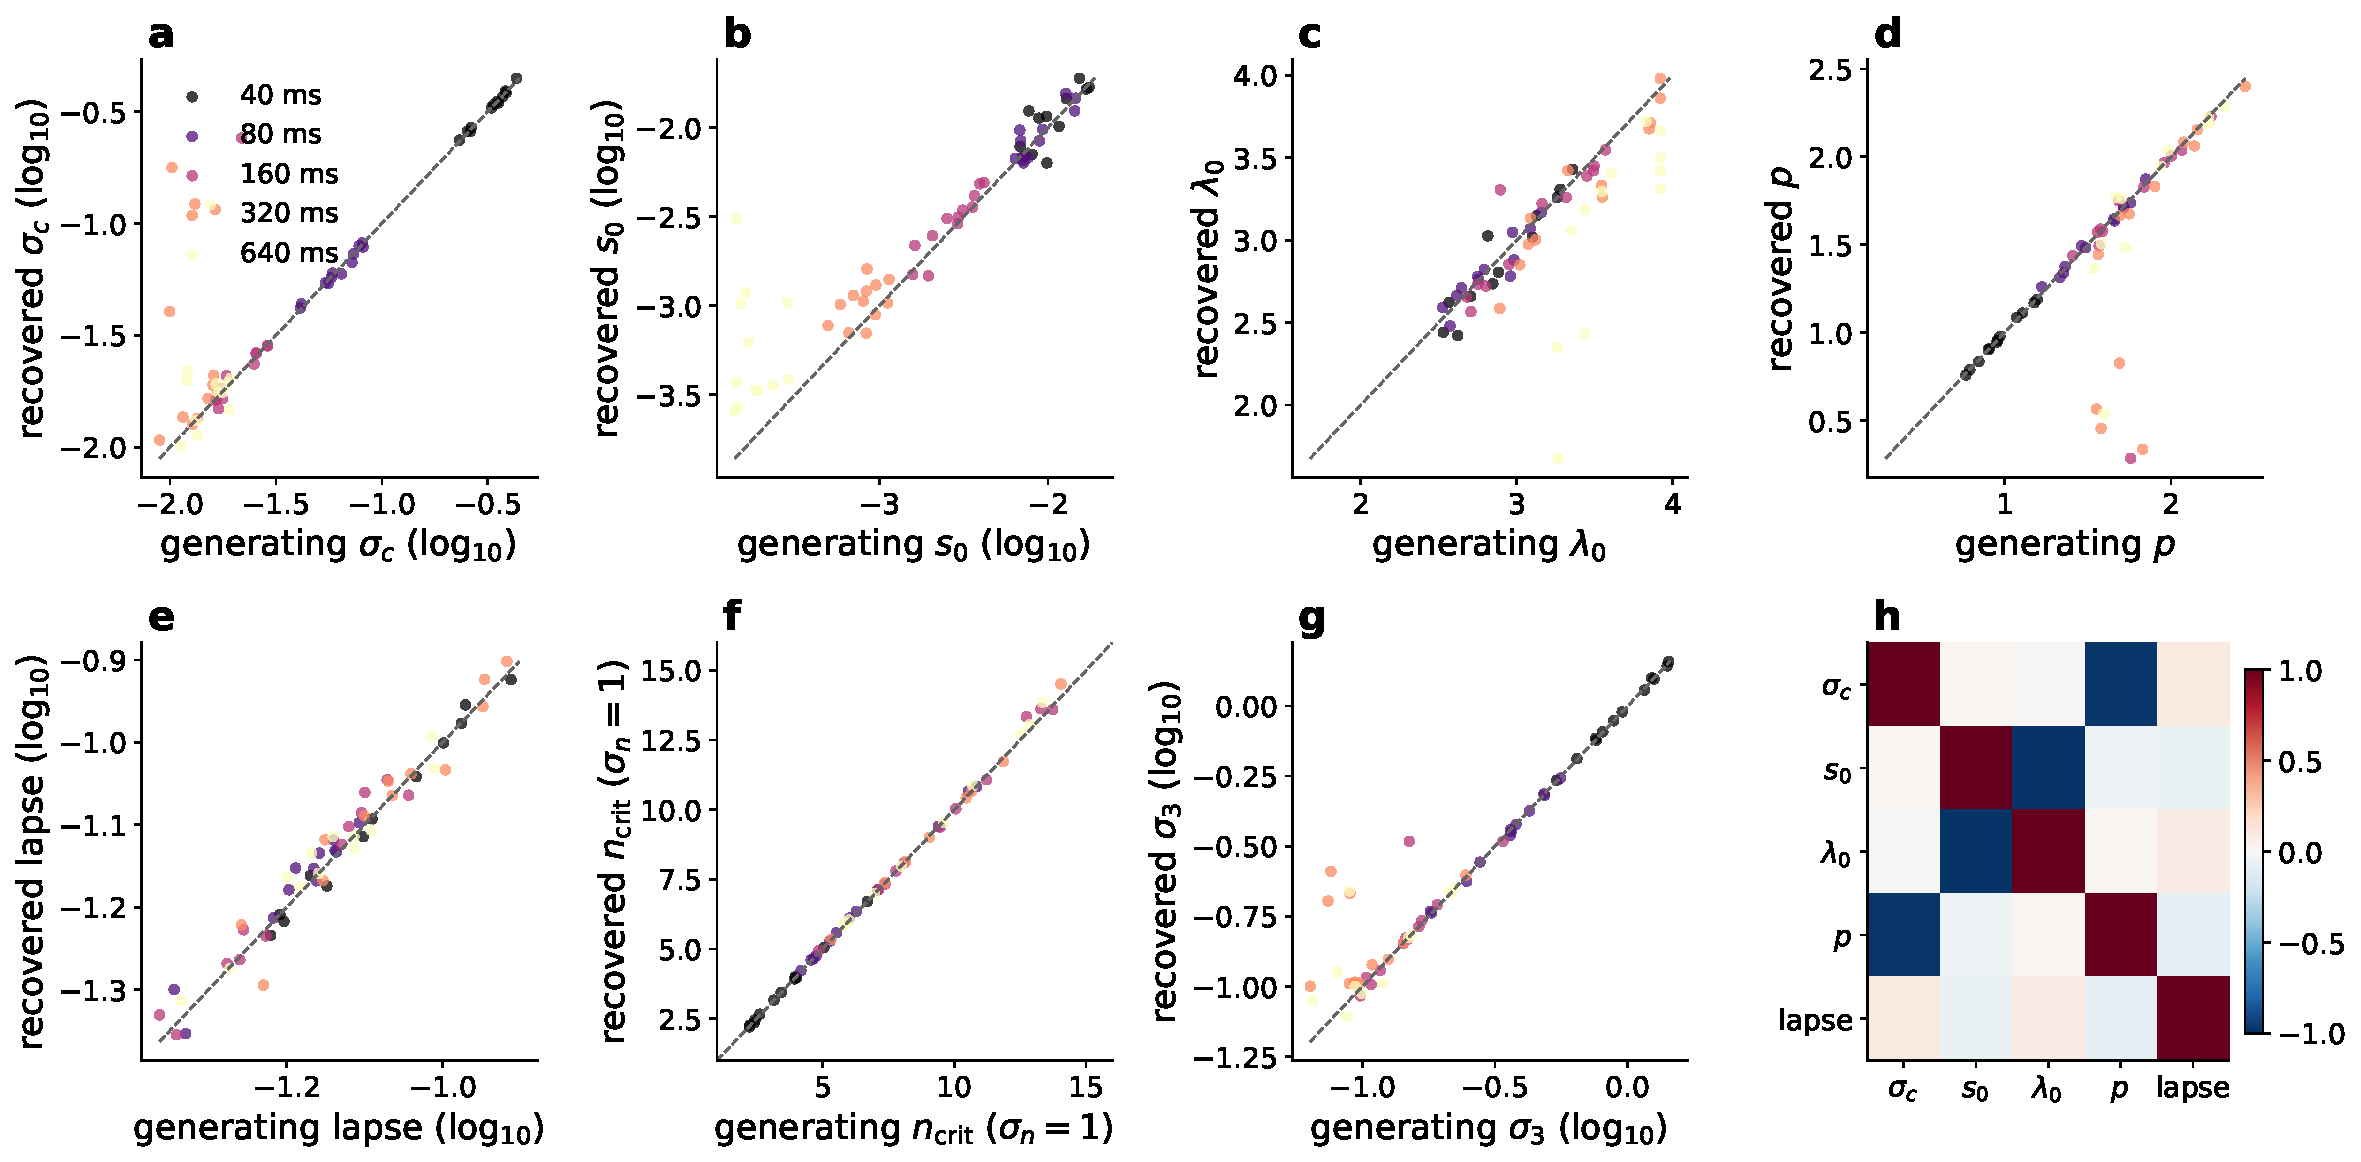
\includegraphics[width=\textwidth]{../output/trial_level_model_comparison/recovery_winner.pdf}
  \caption{\textbf{Parameter recovery of the winning model.} Recovered versus generating values for the five fitted parameters and the derived $n_{\mathrm{crit}}$ and $\sigma_3$, coloured by exposure duration; dashed lines are identity. The bottom-right panel is the Spearman correlation matrix of recovery errors, showing the single strong $s_0$--$\lambda_0$ trade-off.}
  \label{fig:recovery}
\end{figure*}

\section{Supplementary Material 4: The resolution limit \texorpdfstring{$n_{\mathrm{crit}}$}{n\_crit}}
\label{sm:ncrit}

The critical numerosity is defined by adjacent-well discriminability $d' = 1$, i.e.\ $\sigma_n = 1$ (well standard deviation equal to unit spacing)~\citep{macmillan_detection_2004}. Solving $\sigma_n = (\sigma_c/f_n)^\beta = 1$ for the fitted parameters gives $n_{\mathrm{crit}} \approx 4.6,\,7.5,\,8.7,\,9.2,\,10.0$ for 40--640~ms. The crossing lies inside the fitted range at every duration and grows monotonically with exposure (main-text Fig.~\ref{main-fig:comparison}c).

\paragraph{The landscape is intrinsically small-range.} Because the crossing falls inside the fitted window, one might worry that the large-$n$ tail distorts the landscape. It does not: refitting on $n \le 10$ alone returns nearly the same width exponent and $n_{\mathrm{crit}}$ as the full-range fit for 80--640~ms (e.g.\ $\beta = 1.88$ vs.\ $1.81$ at 80~ms, $2.09$ vs.\ $2.19$ at 320~ms; $n_{\mathrm{crit}}$ within $0.3$ at all four), and only the noise-dominated 40~ms flash shifts (Fig.~\ref{fig:ncap}). Within $n \le 10$ the winning model still wins, ahead of its static twin ($\Delta\mathrm{AIC} = 172$) and the Weber/ANS code ($2043$). The exact code is thus a property of the small-number range, not an artefact of fitting the tail.

\begin{figure}[t]
  \centering
  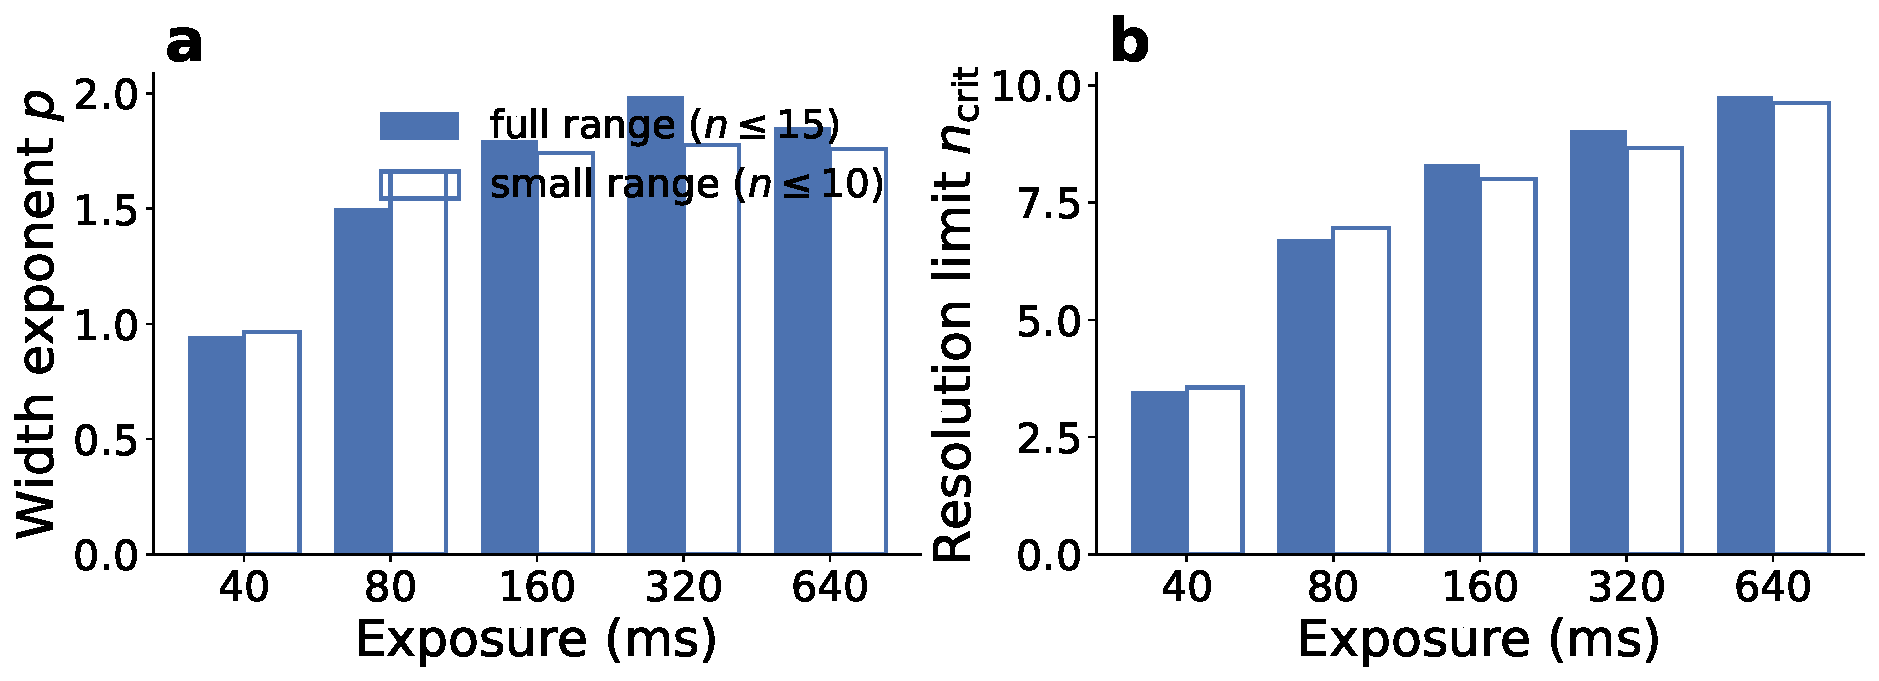
\includegraphics[width=\columnwidth]{../output/trial_level_model_comparison/ncap10_comparison.pdf}
  \caption{\textbf{Small-range refit.} The fitted width exponent $\beta$ (\textbf{a}) and the resolution limit $n_{\mathrm{crit}}$ (\textbf{b}), from the full-range fit ($n \le 15$, filled) and from a refit on the small range ($n \le 10$, open). Both are essentially unchanged for 80--640~ms; only the noise-dominated 40~ms flash shifts. The discrete, exact behaviour is intrinsic to the small-number range.}
  \label{fig:ncap}
\end{figure}

\paragraph{Cross-channel convergence with the response-time plateau.} Within the exact range ($n < n_{\mathrm{crit}}$) the model tracks the geometric-mean response time closely; above it the monotone deliberation-time prediction keeps rising while the empirical RT plateaus, because participants have left the exact regime and are guessing approximately (Fig.~\ref{fig:rtdomain}). The onset of the empirical RT plateau coincides with $n_{\mathrm{crit}}$, which is derived independently from the accuracy channel, a convergence of two channels on the same boundary. We therefore fit the latent-to-seconds RT link on all $n$ and report the within-domain agreement; truncating the fit to $n < n_{\mathrm{crit}}$ is counter-productive, since at short durations the cut falls just before saturation and the truncated fit overshoots.

\begin{figure*}[t]
  \centering
  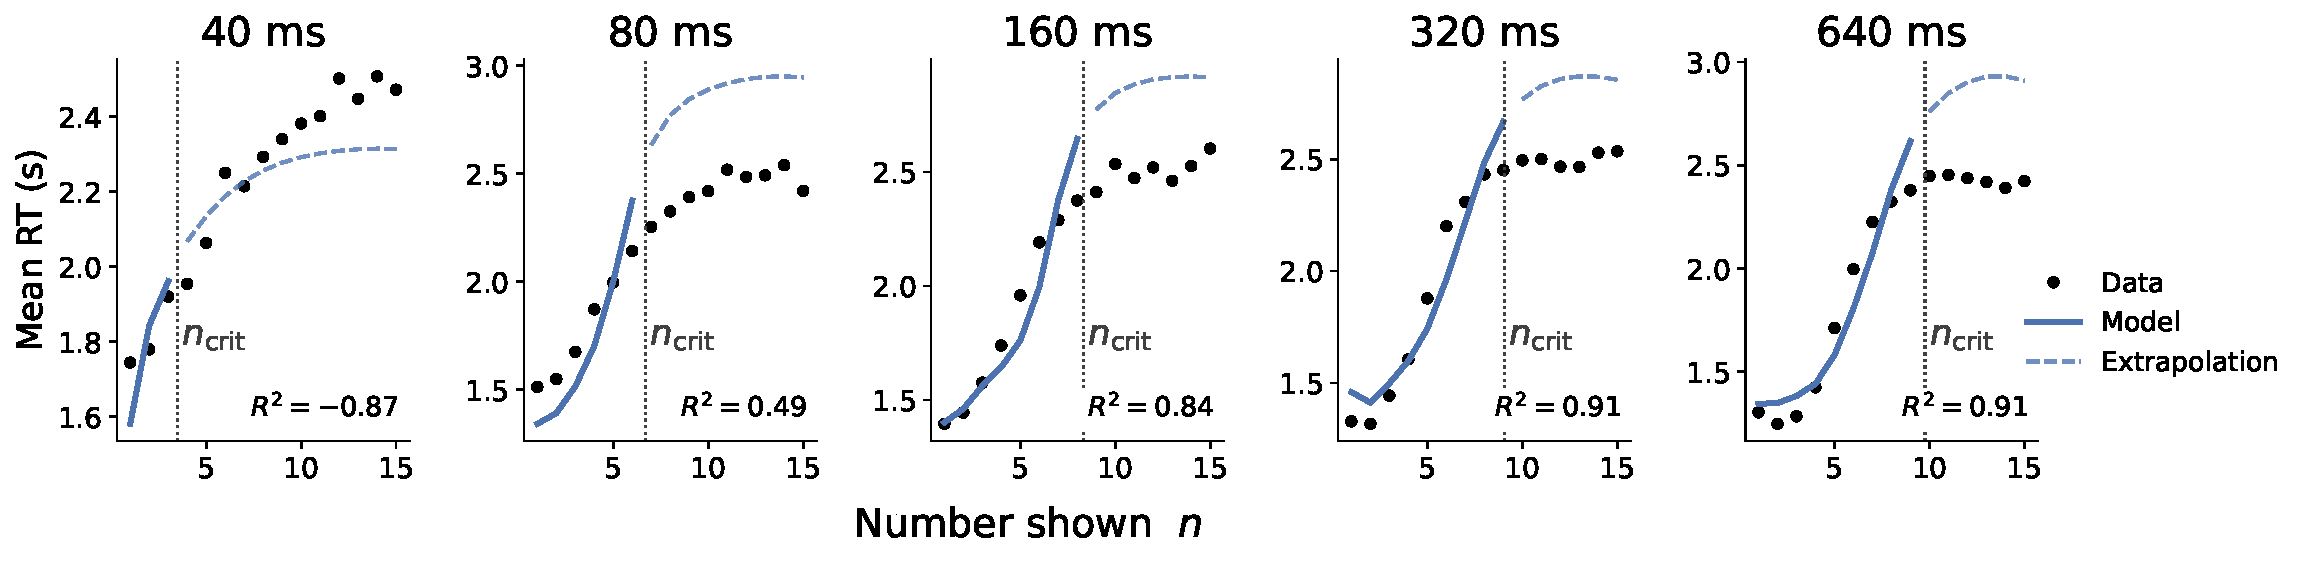
\includegraphics[width=\textwidth]{../output/trial_level_model_comparison/rt_domain.pdf}
  \caption{\textbf{Response time within and beyond the exact range.} Predicted geometric-mean RT (solid, $n < n_{\mathrm{crit}}$; dashed, extrapolated above) against the data. Within the exact range the model tracks RT; above $n_{\mathrm{crit}}$ it over-predicts, the signature of the switch to approximate responding. The RT plateau onset coincides with the independently derived $n_{\mathrm{crit}}$.}
  \label{fig:rtdomain}
\end{figure*}

\paragraph{The discrete signature in exact accuracy.} The four-parameter landscape is smooth, yet the predicted proportion of exact responses shows a small shoulder in the subitizing range. This is not extra fitted flexibility: it is the discrete clean-up basins on the fixed integer lattice, and it vanishes when the clean-up is switched off (Fig.~\ref{fig:pexact}). The wiggle is thus a signature of the mechanism rather than of additional degrees of freedom.

\begin{figure}[t]
  \centering
  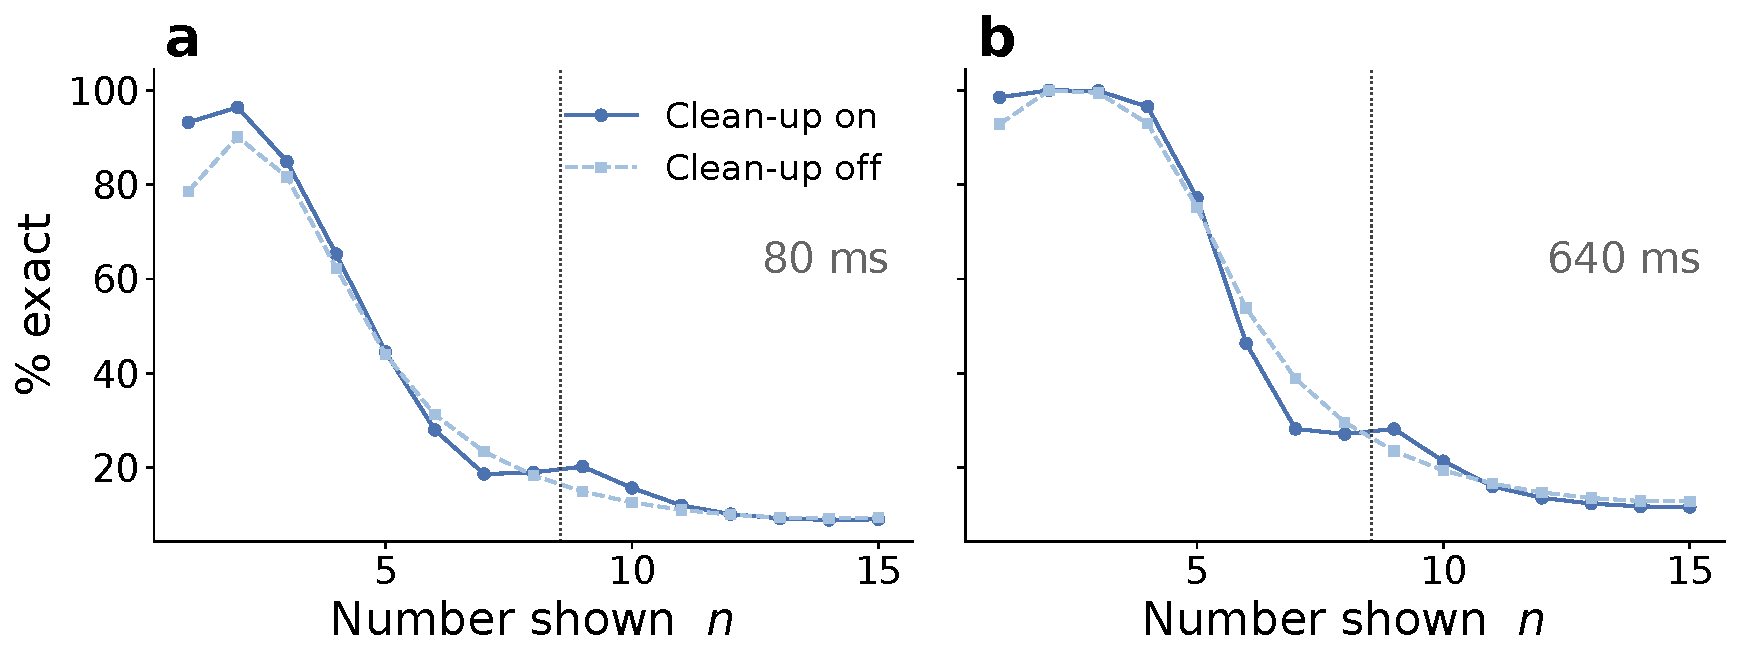
\includegraphics[width=\columnwidth]{../output/trial_level_model_comparison/pexact_decomposition.pdf}
  \caption{\textbf{The exact-accuracy shoulder is a clean-up signature.} Top: the fitted well-width and sensory-noise profiles are smooth. Bottom: the proportion of exact responses shows a discrete shoulder with clean-up on (solid) that disappears with clean-up off (dashed), the discrete basins on the integer lattice, not extra parameters.}
  \label{fig:pexact}
\end{figure}

\paragraph{The effective Weber fraction.} We computed the coefficient of variation (CoV) of the model's fitted response distribution --- $(1-\ell)\,p(r \mid n) + \ell/R_{\max}$, the model exactly as fitted, with the lapse included --- per numerosity and exposure, restricted to the in-support range so that it is the like-for-like counterpart of the empirical estimates, and overlaid the empirical CoV (Fig.~\ref{fig:weber}). The model tracks the data across the whole range at every exposure. The CoV is elevated at the smallest numerosities (where the ratio $\mathrm{sd}/\mathrm{mean}$ is inflated by the small denominator, in model and data alike) and settles to a roughly constant plateau across the estimation range ($n \ge n_{\mathrm{crit}}$). A power-law fit $w_{\mathrm{eff}} \propto n^{\gamma}$ over the estimation range gives a pooled exponent $\gamma \approx -0.2$ for both the model ($-0.21$) and the data ($-0.17$): approximately scalar variability, close to the Weber value $\gamma = 0$ and far from the $1/\sqrt{n}$ decline ($\gamma = -0.5$) that a Poisson magnitude code would predict. The model thus reproduces the measured variability, and its slope, across the estimation range --- one landscape accounting for numerosity variability in both regimes.

\begin{figure}[t]
  \centering
  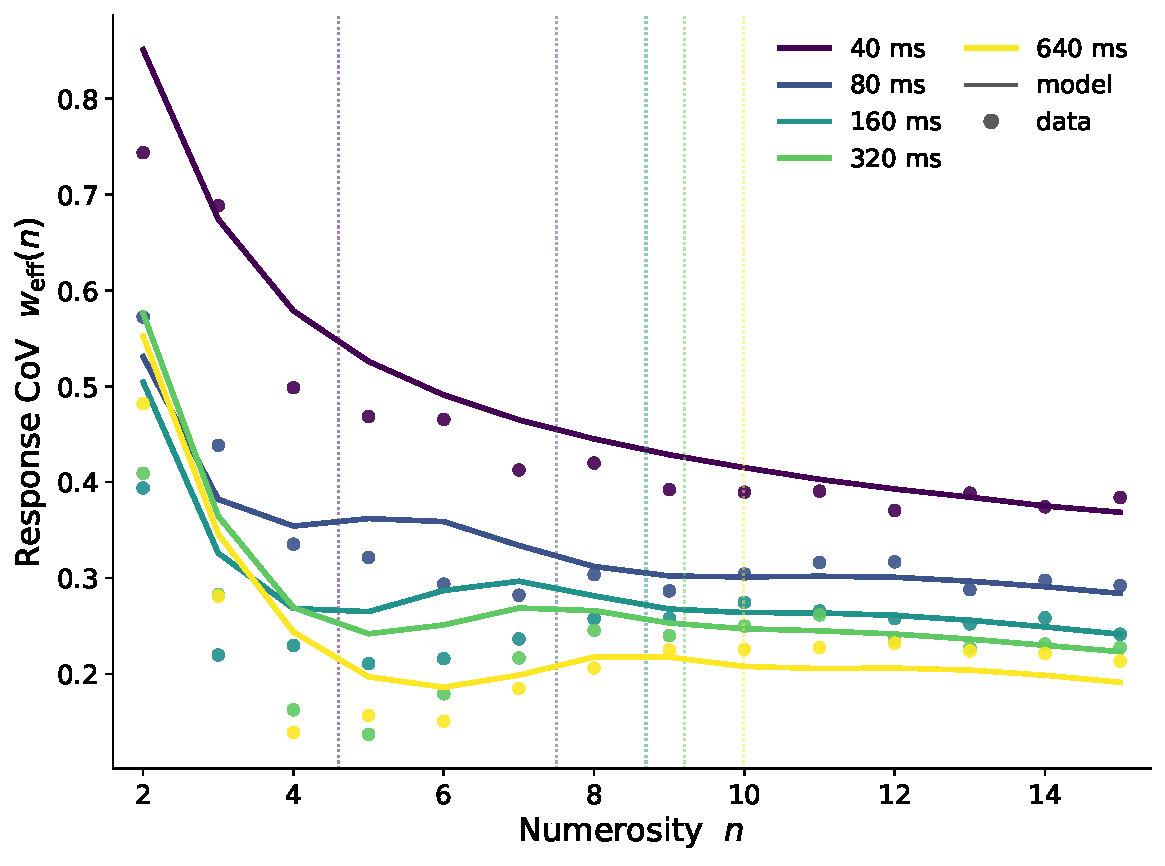
\includegraphics[width=\columnwidth]{../output/trial_level_model_comparison/weber_fraction.pdf}
  \caption{\textbf{The effective Weber fraction.} Coefficient of variation of the response distribution $w_{\mathrm{eff}}(n)$ per numerosity, for each exposure duration; solid lines are the model (the fitted response distribution, lapse included, restricted to in-support and renormalised), dots the data (in-support responses), and dotted verticals mark $n_{\mathrm{crit}}$. The model tracks the data across the whole range; across the estimation range ($n \ge n_{\mathrm{crit}}$) the CoV settles to a roughly constant plateau, approximately scalar variability (Weber's law). The 40~ms flash is noise-dominated and has no exact range.}
  \label{fig:weber}
\end{figure}

\section{Supplementary Material 5: Exploratory reanalysis of developmental dyscalculia}
\label{sm:dyscalculia}

As an exploratory extension we applied the winning model to the exact-enumeration data of~\citet{decarli_impaired_2020}: accuracy and response time per subject and numerosity for $32$ children with developmental dyscalculia (DD) and $32$ age-matched controls, using numerosities $n = 1$--$7$ (dropping $n = 8$ exactly as the original authors do, for the guessing end-effect they report). The winning model fits both groups well and independently prefers a super-linear width ($\beta \approx 1.5$--$1.6$), a cross-dataset replication, with a re-derived $n_{\mathrm{crit}}(\sigma_n = 1) \approx 8$, a plausible resolution limit for exact enumeration. The argument has three tiers, strongest-anchored first (Fig.~\ref{fig:decarli}).

\emph{Model-agnostic deficit.} DD are ${\approx}10\%$ less accurate at $n = 4$--$6$ (Cohen's $d = -0.62$) and ${\approx}0.3$~s slower at $n = 4$--$7$ ($d = +0.61$), with the difference concentrated at $n = 4$ (Mann--Whitney $p = 0.001$), the subitizing edge, not a uniform slowdown. This needs no model.

\emph{The deficit is resolution-shaped, not noise-shaped.} With an exhaustive per-subject grid search and a fixed common lapse, a single-mechanism \emph{resolution} model (well merging, sensory noise off) fits each subject's accuracy curve far better than a single-mechanism \emph{noise} model (well width off): $64/64$ subjects, mean SSE $0.010$ vs.\ $0.079$, Wilcoxon $p = 3.5\times10^{-12}$. The exact-enumeration decline is a discrete-resolution phenomenon, which both validates the attractor framework on independent data and says where the group effect must live.

\emph{The group difference localises to resolution.} Per-subject, the resolution limit is shorter in DD ($n_{\mathrm{crit}} = 8.2$ vs.\ $9.1$ for controls; Mann--Whitney $p = 0.004$ with the RT channel included). Sensory noise shows only a weak trend ($p = 0.07$) and fits worse. The standardised $n_{\mathrm{crit}}$ effect ($d = -0.65$) matches the raw accuracy effect, so the modest raw shift of ${\approx}0.9$ numerosities is a units effect, not a small one.

\begin{figure}[t]
  \centering
  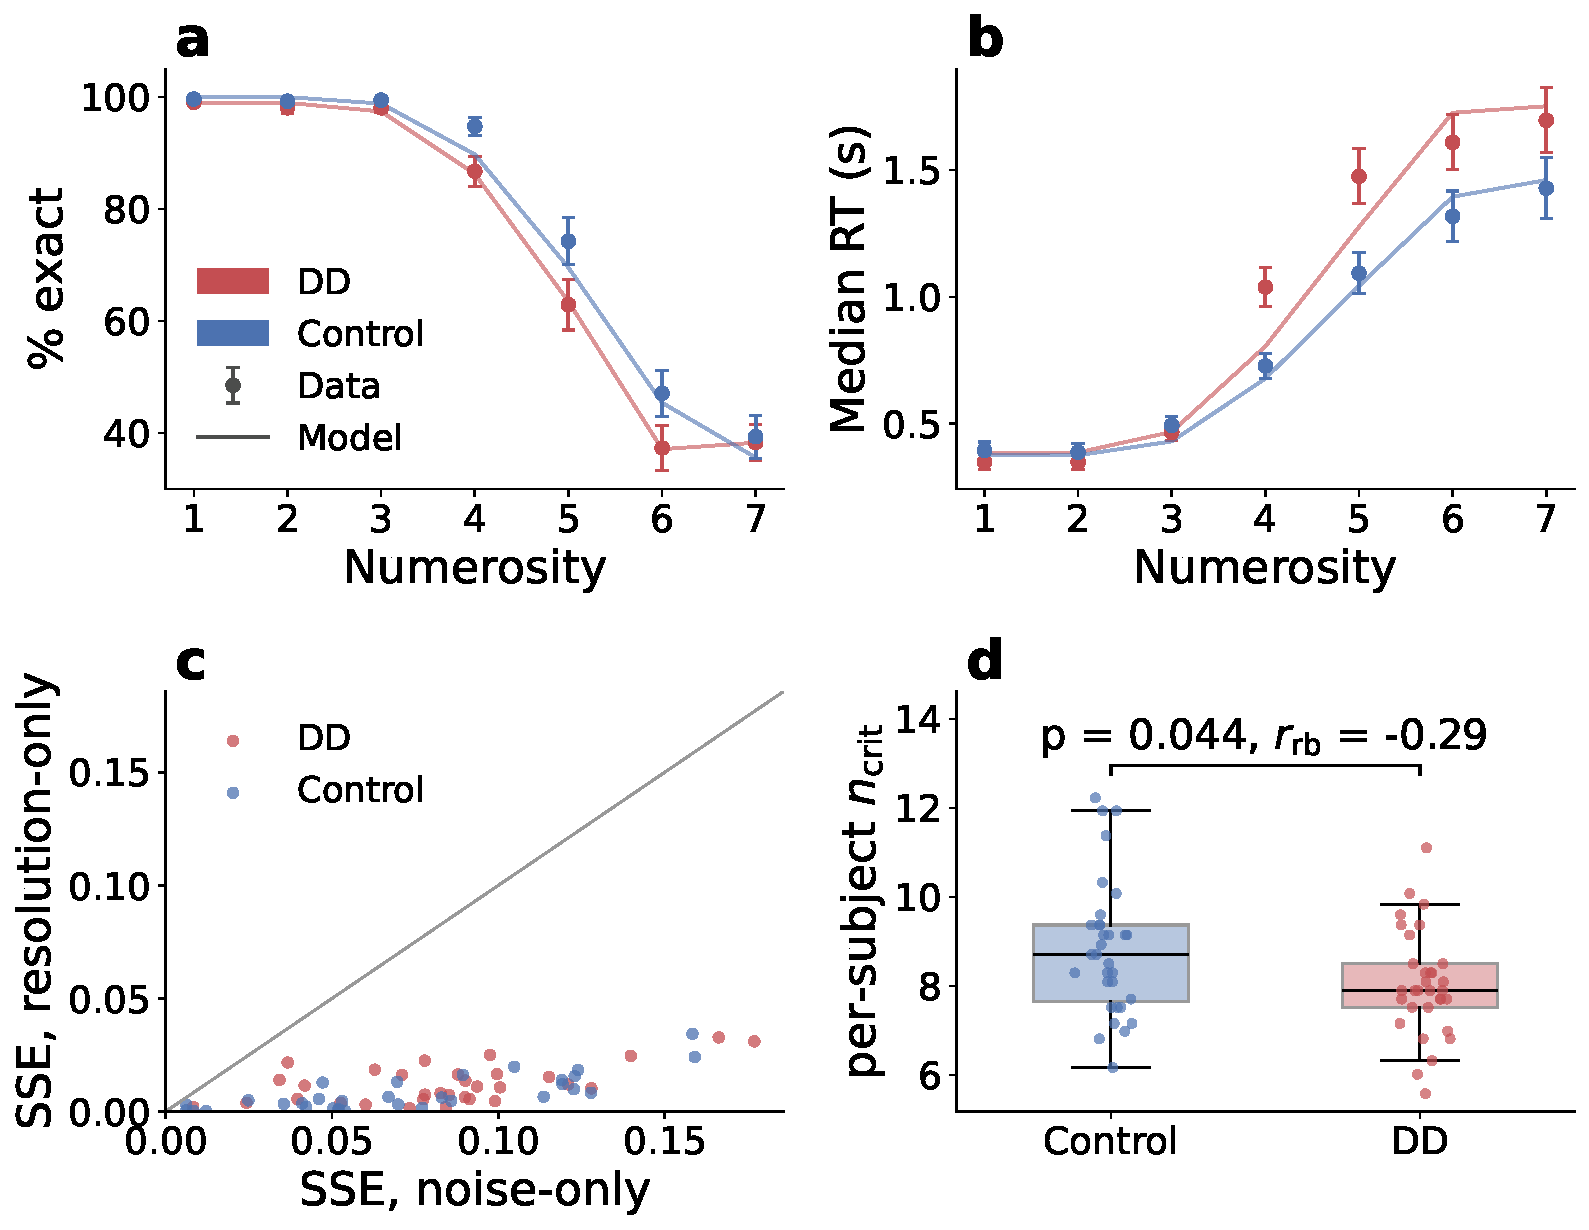
\includegraphics[width=\columnwidth]{../output/decarli_fit/decarli_dd_summary.pdf}
  \caption{\textbf{Developmental dyscalculia as a shorter exact number code.} (a)~Exact accuracy: DD are less accurate, concentrated at $n = 4$ (${**}$). (b)~Response time: DD are slower in the transition band. (c)~A resolution model fits each subject's accuracy better than a noise model ($64/64$; below the diagonal). (d)~The per-subject resolution limit $n_{\mathrm{crit}}$ is shorter in DD.}
  \label{fig:decarli}
\end{figure}

The reading for the paper is that developmental dyscalculia is, on this model, \emph{not} a noisier perception of number but a coarser, shorter exact code: the discrete resolution runs out earlier, right at the subitizing edge. This is a specific, mechanistic, falsifiable claim, though much of the statistical power comes from analysing subjects individually rather than at the group level, not from the model alone. It is complementary to the account of~\citet{dolfi_weaker_2024}, who locate the dyscalculic deficit in a weaker number sense within an image-computable network: both find the deficit in the number code, and coupling our attractor to such a front end (the present model sets the front end aside) is the natural way to ask whether a resolution deficit and a sensory-noise deficit can be told apart in the same model. The analysis remains exploratory: the data are coarse ($8$ trials per cell), the resolution-versus-noise localisation is a lean supported by the decisive per-subject model comparison rather than a full identification, and a small sensory-noise component may coexist.

% Uncomment when you need citations from the shared bibliography:
\bibliographystyle{SageH}
\bibliography{references}

\end{document}
